\documentclass[10pt,a4paper]{article}
\usepackage[margin=16mm]{geometry}\usepackage{fontspec,amsmath,graphicx,booktabs}
\setmainfont{Latin Modern Roman}\setlength{\parindent}{0pt}\setlength{\parskip}{6pt}
\begin{document}
{\Large Gain calibration followed by soft recovery-domain penalties}\par 6 October 2026

One relative gain correction was estimated from pooled training-average bins, before the unchanged inverse transmission matrix. Multipliers on historical inverse gains, in $(0,90,45,135)$ order: $(0.992729,1.005313,1.009114,0.992952)$. Their product is one to fix the overall scale. Separate-window estimates differ by at most about 0.37 percentage points. This is pair-balance calibration conditional on the common-field optical model, not independent detector calibration; offsets and matrix errors were not fitted.

Held-out measured pair-imbalance RMS changes from 0.375\% to 0.302\% (30--31 s), and 0.320\% to 0.303\% (10--11 s). Gain therefore explains only part of the imbalance. Existing accepted cycles and original bins are retained; the new calibration is applied linearly to those channel means, then uniform final-arc references and held-out interpolation weights are rebuilt from training data. Historical gain corrections are not applied twice.

Signal, coherent background, noninterfering Stokes background and cross term each obey pair balance by construction in this model. Gains are frozen before fitting. No extra pair-sum penalty is needed to impose those model identities; data imbalance remains part of the four-channel residual. Richard's four independent coefficients would require a separate restricted parameterization or explicit pair penalty and were not refitted here.

For each training point, $\widehat S=I^{train}-B-L(d^{fit})$. The objective is
\[
J=\sum_{ij}(\varepsilon_{ij}/T_j^{train})^2
+w\sum_j[\max(0,\widehat r_j/r_{max}-1)]^2
+w\sum_{ij}[\min(0,\widehat S_{ij})/T_j^{train}]^2.
\]
No signal-relative residual weighting is used. In the radial penalty only, pair denominators have a numerical floor $10^{-4}T_j^{train}$ to avoid division by zero; negative channels are penalized separately. Physical inversion and reported invalid counts use unmodified corrected channels. These soft squared-hinge penalties allow finite exceedance. Weight values are sensitivity choices, not experimentally calibrated tolerances.

High- and lower-background starts were checked. Penalized selected fits use 8192 curve intervals; all selected fits converged. The same single stationary field is shared across windows. No parameter selection used held-out outcomes.

\begin{tabular}{llrrrr}\toprule
Weight & Window & Train invalid & Test invalid & Test RMS & Max test $r-r_{max}$\\\midrule
0 & 30s & 21 & 23 & 0.00503 & 3.6635 \\
0 & 10s & 0 & 23 & 0.00953 & 2.1164 \\
0.01 & 30s & 19 & 21 & 0.00507 & 0.4743 \\
0.01 & 10s & 0 & 22 & 0.00962 & 0.6639 \\
0.1 & 30s & 17 & 20 & 0.00502 & 0.4748 \\
0.1 & 10s & 0 & 18 & 0.00964 & 0.6665 \\
1 & 30s & 11 & 15 & 0.00493 & 0.5829 \\
1 & 10s & 0 & 19 & 0.00968 & 0.7295 \\
10 & 30s & 4 & 9 & 0.00490 & 0.6613 \\
10 & 10s & 0 & 18 & 0.00971 & 0.7604 \\
\bottomrule\end{tabular}

Invalid includes negative channels and radial exceedance, even a tiny exceedance. Max excess is floored at zero. Counts alone do not measure violation size. The penalty is applied to training data only; it cannot guarantee physically invertible held-out corrections. These are conditional fitted-cross-term subtraction diagnostics, not independent field inversions or absolute angle validation.
\newpage
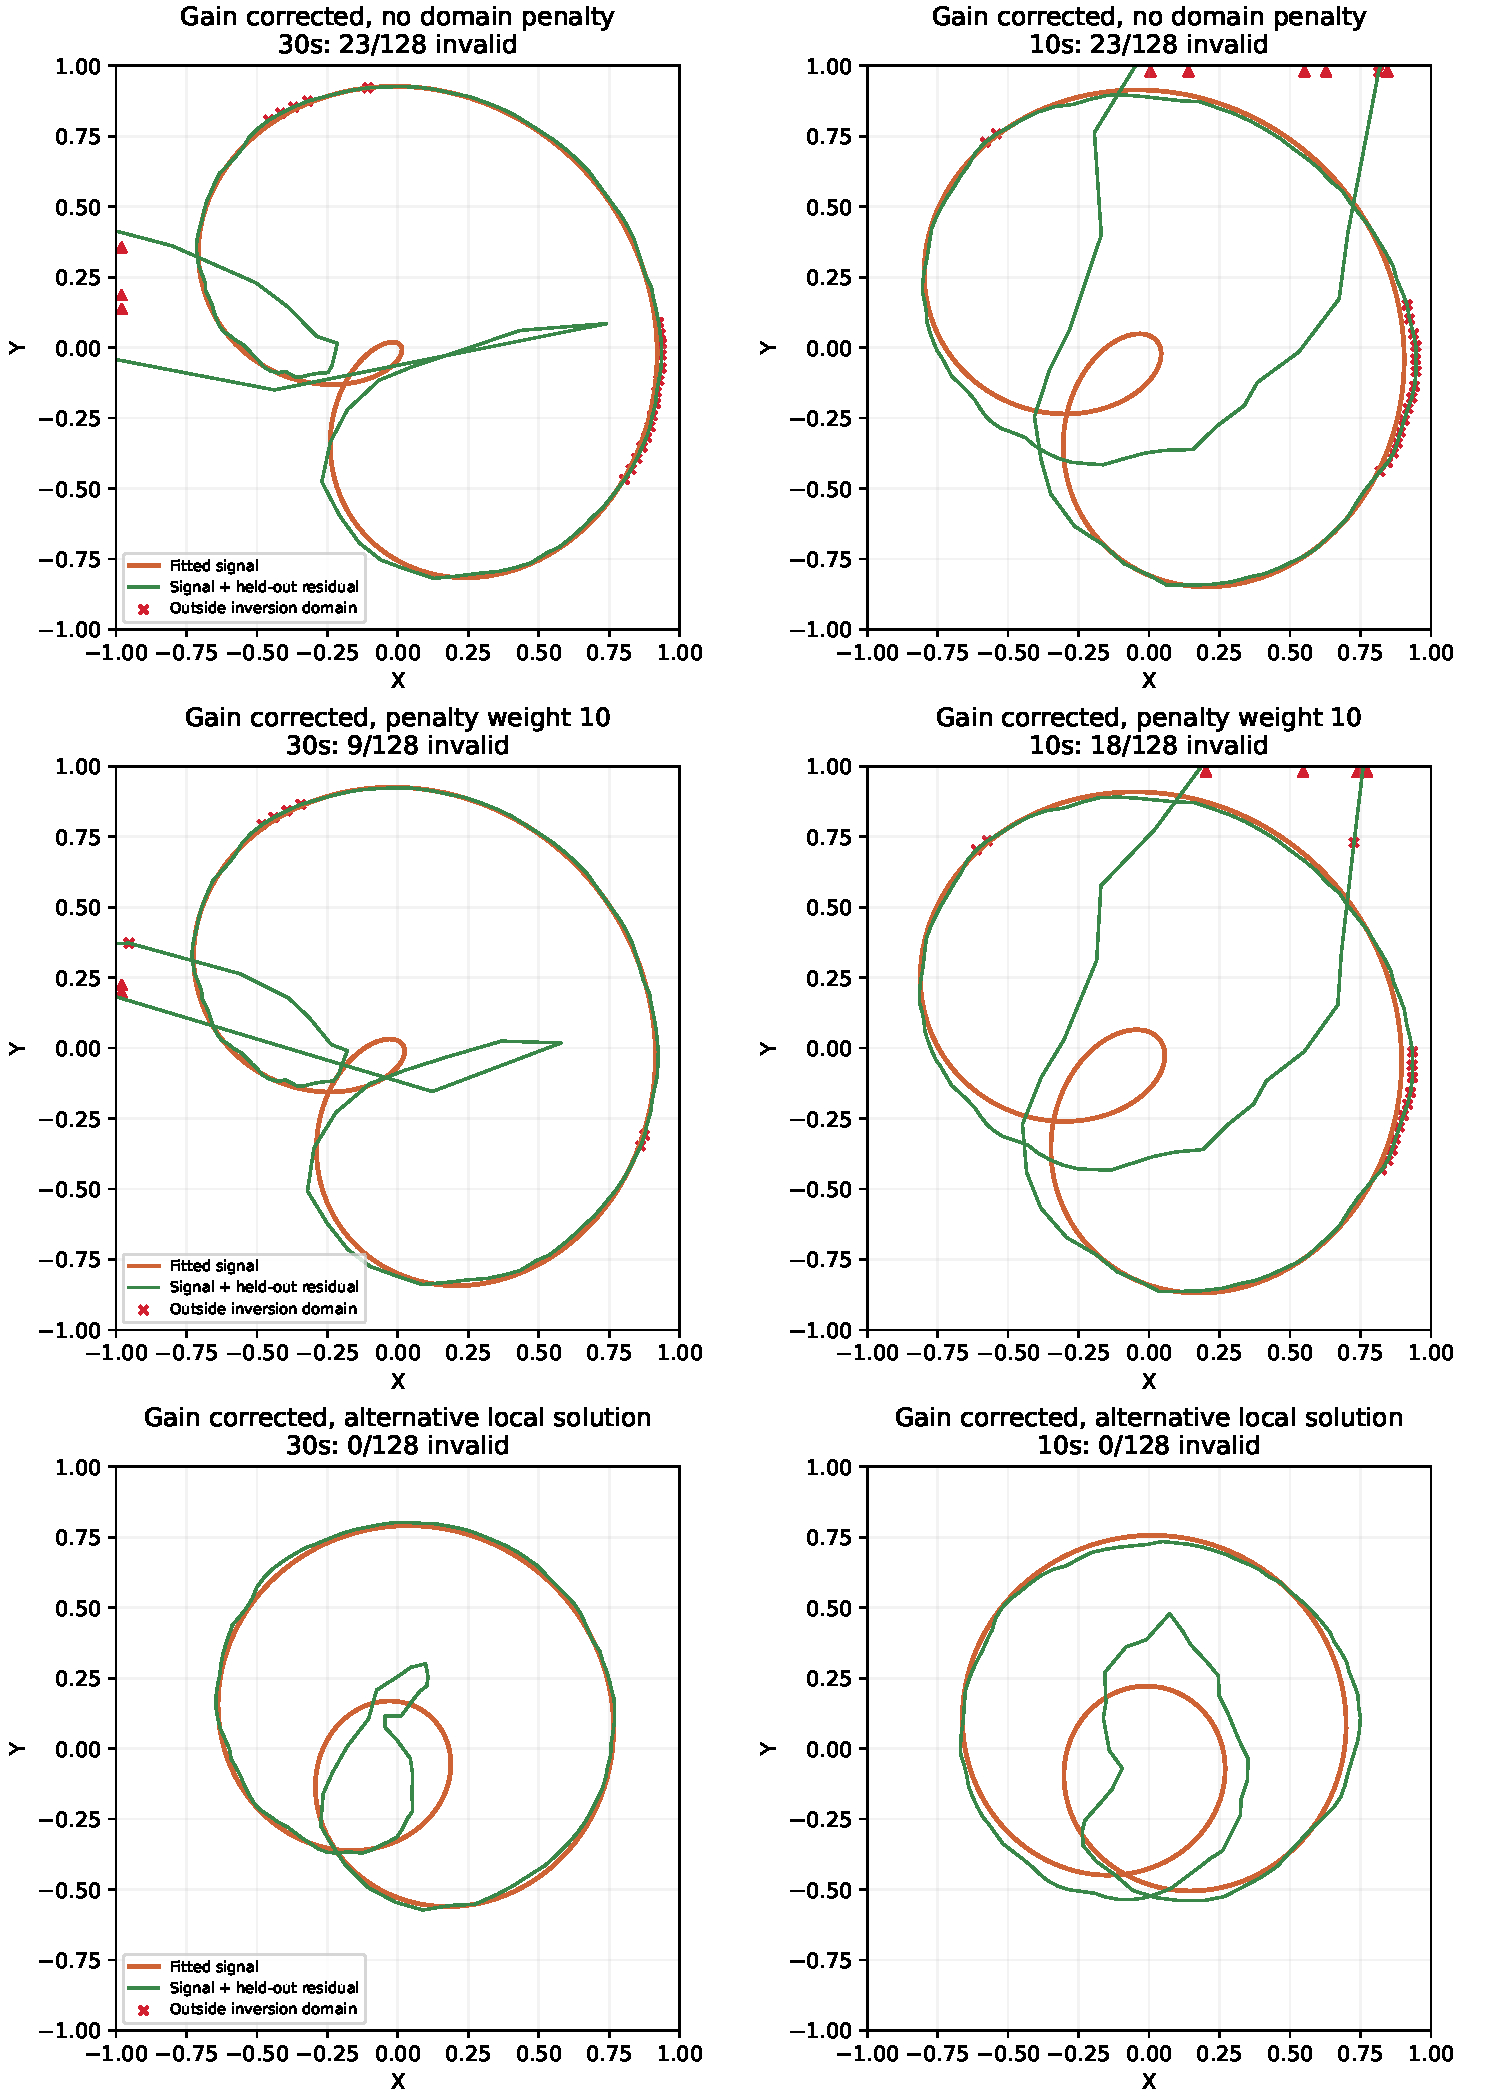
\includegraphics[width=\linewidth,height=.94\textheight,keepaspectratio]{comparison.pdf}
\end{document}
